\section{Simulator in Matlab}\label{sec:matlab_simulator}

This Matlab landmark sensing simulator was realized in order to generate a sequence of observations subjected to noise to be provided at the SLAM.
The simulator provides a GUI that allows the user to navigate in a map filled with randomly-placed landmarks, and visualize in real-time both the real 
and the noised configurations sequences. Gaussian noise is added in order to consider the uncertainties on robot perceptions originated from physical process
like wheels slippage or sensor noise.\\
The simulator produces as output a text file where is associated a sequence of robot's states and the landmarks perception from these states.

\subsection{Configuration representation}
A robot configuration $C$ is represented by the mean of a 2D homogeneous matrix (at the $k-th$ simulator iteration):

\[ 
\textbf{C}(k) = 
\left( \begin{array}{c:c}
  \textbf{R}(k)  & \textbf{t}(k) \\ \hdashline
  0 & 1  \\
\end{array} \right)
\]
with $\textbf{t} = [x,y]^T$.\\
The matrix also represents univocally a certain state of the robot $[x,y,\theta]$.
\\
The robot model used is a planar unicycle, with two control inputs (linear and angular velocity) controllable by human user.
The robot is equipped with a sensor capable of returning the bearing of all landmarks within a certain distance $r$.\\
The instantaneous linear velocity $v \in \mathbb{R}$ is directed in the $x$ (sagittal) axis of the robot, while angular velocity $\theta \in \mathbb{R}$ is
around the $z$ axis of the workspace (orthogonal to the plane). Of course this values are intended to be deduced from the encorders on the wheels.\\
Given a certain configuration $\textbf{C}$(\textit{k}) and the two instantaneous velocities $v$ and $\theta$, the configuration at the next iteration is computed as:\\
\vspace{1 cm}
\[ 
\textbf{C}(k+1) = 
\left( \begin{array}{c:c}
  %%\textbf{R(k)} * \textbf{H_r}  & \textbf{t(k)} + \textbf{\tilde{t}} \\ \hdashline
  \textbf{R}(k) \cdot \textbf{H}_r & \textbf{t}(k) + \tilde{\textbf{t}} \\ \hdashline
  %%\textbf{R(k)}  & \textbf{t(k)} \\ \hdashline
  0 & 1  \\
\end{array} \right)
\]
\[ 
\tilde{\textbf{t}} = [\tilde{t_x},\tilde{t_y}]^T = \textbf{R}(k) \cdot [v,0]^T
\]

\[ 
\textbf{H}_r =
\left( \begin{array}{cc}
  cos(\theta)  & -sin(\theta)\\ 
  sin(\theta)  & cos(\theta) \\
\end{array} \right)
\]\\

This model is equivalent to the unicycle in ``Robotics, modelling, planning and control'' ([Siciliano, Sciavicco, Villani, Oriolo], 2008).
Note that the integration method used for an ideal unicycle is the \textit{approximated Euler}, since we are considering that the $\theta$ remains constant during the integration step,
and changes suddenly at the next step (instead of changing continuously as it would be in reality).\\
\subsection{Configurations storing}
The \textit{distance} $d$ between two configuration matrices $M_1$, $M_2$ representing respectively states $~ s1 = [x_1,y_1,\theta_1]$,$~ s2 = [x_2,y_2,\theta_2]~$
is defined as
\[ 
d = \alpha \cdot d_{\theta} + d_p
\]
where $d_{\theta}$ is the absolute value of the the (circular) distance between angles $\theta_1$,$\theta_2$,
and $d_p$ is the norm of the vector $[x_1 - x_2,y_1 - y_2]^T$.\\
The parameter $\alpha$, usually bigger than $1$, balances the importance of the rotation component respect the linear one.\\
While user navigation proceeds the simulator stores in two separete lists (real and noised) the subsequent configurations $\textbf{C}$.
At a certain iteration, both current noised and real configurations are appended to their lists if and only if the \textit{distance} between the current noised configuration 
and the last saved noised configuration exceeds a certain threshold (this models an on-board robot software that can dispose only of the noised perceptions).\\
%%These two list are used to provide the user in real time the comparison between real and noised configurations.
\\
\begin{figure}[htbp]
  \centering
    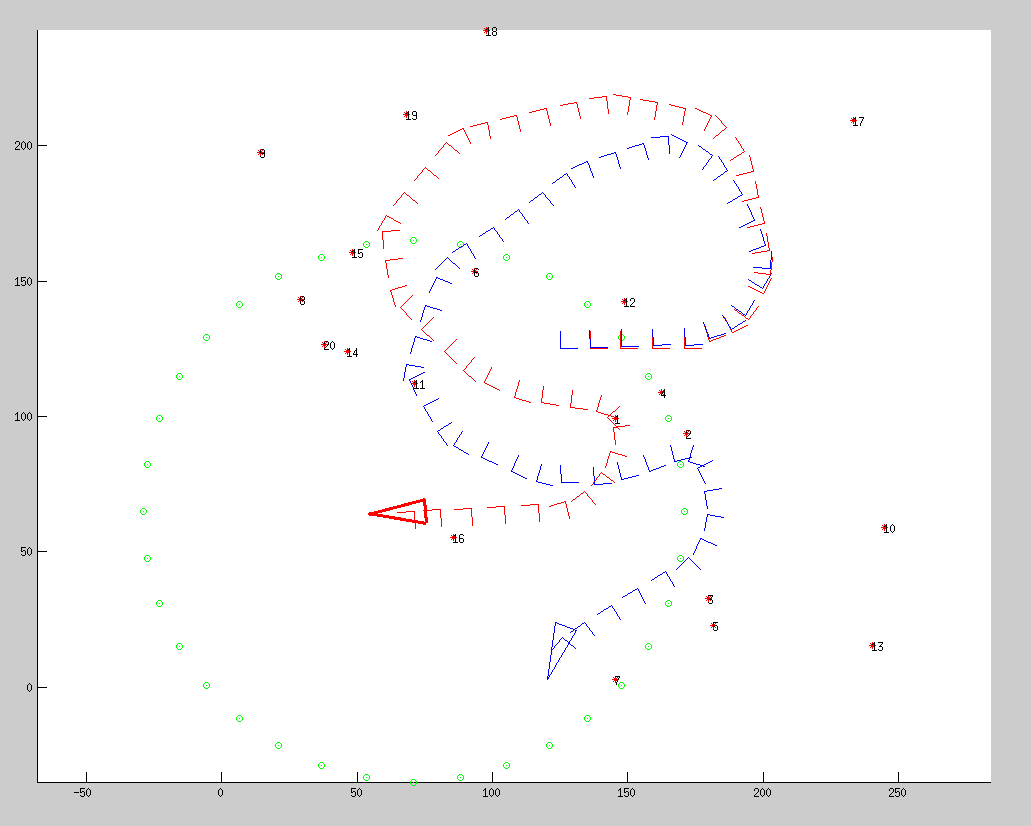
\includegraphics[width=0.8\textwidth]{images/matlab_simulator.png}
  \caption{GUI represents both real (red) and noised (blue) configuration sequences.}
  \label{fig:matlab_simulator}
\end{figure}

\vspace{1 cm}
\subsection{Landmark readings}
Every time that a configuration is appended to its list, a new \textit{landmark reading} is appended at the simulator's output file.
A \textit{landmark reading} is composed by two rows with a certain number of fields:\\\

$
odomPose, ~~ ID, ~~ n_X, ~ n_Y, ~  n_{\theta}, ~  t_X, ~  t_Y, ~ t_{\theta}
$\\

$
bearing, ~~ b_1, ~ ... ~ b_n, ~ IDb_1, ~ ... ~ IDb_n, 
$\\ \\
where:
\textit{$ID$} is the identificative number of the reading, $[n_X, n_Y, n_{\theta}]$ is the noised state of the robot, $[t_X, t_Y, t_{\theta}]$ the real one.
The $n$ values $ b_1 ... b_n$ gives the bearing angle of the $n$ landmarks visible from $[t_X, t_Y, t_{\theta}]$. The $i-th$ bearing value is then associated to 
the relative landmark's identificative number $IDb_i$.
The n landmarks are the perceptible one, that means that are within a certain constant distance $r$ from position $[t_X, t_Y ]$.


\subsection{Odometry and sensors noise}
The error on the odometry is modeled as a zero-centered white noise with gaussian distribution, that influences independently the two velocities $v$ and $\theta$.
The standard deviation of the distribution has a constant component and an additional component that is directly proportional to the norm of velocity $v$ or $\theta$.
This models the fact that in reality we usually tend to have higher odometric errors with higher robot wheels velocities.
\\
The error on the bearing sensor is modelled as a zero-centered white noise with gaussian distribution, that is directly summed to the bearing readings.\\
